\section{Optimierung}
\subsection{Graphische Methoden}
\subsubsection{Sprague Grundy}
\begin{tabularx}{\textwidth}{XX}
	\vspace{-4cm}
\begin{enumerate}
	\item Endknoten (Verlierpositionen) haben Rang 0
	\item Von jeder Gewinnerposition führt mind. ein Pfeil auf einen Rang 0 Knoten
	\item Alle Pfeile von einem Knoten mit Rang 0 führen zu einem Knoten mit Rang $>$ 0
\end{enumerate} &
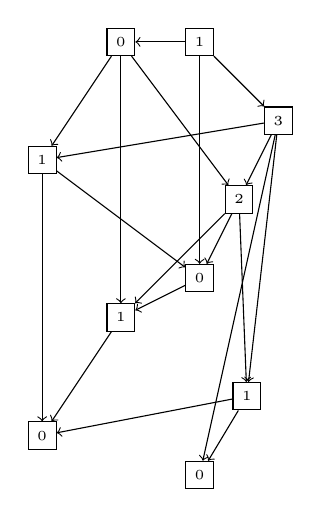
\begin{tikzpicture}[font=\tiny]
	\node (a) at (1,0) [draw]{0};
	\node (b) at (2,0) [draw]{1};
	\node (c) at (3,-1) [draw]{3};
	\node (d) at (0,-1.5) [draw]{1};
	\node (e) at (2.5,-2) [draw]{2};
	\node (f) at (2,-3) [draw]{0};
	\node (g) at (1,-3.5) [draw]{1};
	\node (h) at (2.6,-4.5) [draw]{1};
	\node (i) at (0,-5) [draw]{0};
	\node (j) at (2,-5.5) [draw]{0};

	\draw[->] (a)--(d);
	\draw[->] (a)--(e);
	\draw[->] (a)--(g);

	\draw[->] (b)--(a);
	\draw[->] (b)--(c);
	\draw[->] (b)--(f);

	\draw[->] (c)--(d);
	\draw[->] (c)--(e);
	\draw[->] (c)--(h);
	\draw[->] (c)--(j);

	\draw[->] (d)--(f);
	\draw[->] (d)--(i);

	\draw[->] (e) -- (h);
	\draw[->] (e) -- (f);
	\draw[->] (e) -- (g);

	\draw[->] (f) -- (g);

	\draw[->] (g) -- (i);

	\draw[->] (h) -- (i);
	\draw[->] (h) -- (j);
\end{tikzpicture}
\end{tabularx}

\subsection{Lagrange}
Lagrange Multiplikatoren definieren Nebenbedingungen:\\
\begin{tabular}{l l l}
	{$ h(x,\lambda) = f + \sum\limits_{k=1}^s{\lambda_k g_k} $ } &
		$s$:    &Anzahl Nebenbedingungen \\
		&$f(x)$:&Zu optimierende Funktion \\
		&$g_k$: &Nebenbedingungen mit $g_k(x) = 0$
\end{tabular}
\subsubsection{Beispiel}
Auf der Funktion $f(x,y) = x^2 + y^2$ ist der tiefste Punkt zu finden,
für den gilt: $y = 3x - 5$ \\
$ h(x,y,\lambda) = x^2 + y^2 + \lambda(y - 3x + 5) $ \\
Partielle Ableitungen $h'(x,y,\lambda)$ Null setzen
\begin{tabular}{ll}
	$f'(x)$&$ = 2 x + 3 \lambda$ \\
	$f'(y)$&$ = 2 y + \lambda$ \\
	$f'(\lambda)$&$ = y - 3x + 5$
\end{tabular}

Dieses Gleichungssystem kann dann ganz normal aufgelöst werden.

\subsection{Lineare Optimierung}
\subsubsection{Gradientenabstieg} \label{2_Gradientenabstieg}
\begin{enumerate}
	\item Startpunkt wählen
	\item Entlang des steilsten Abstiegs entlang bis Steigung zunimmt
	\item Neu ausrichten und wiederholen
	\item Fertig wenn Gradient nach unten zeigt
\end{enumerate}
Der Gradientenabstieg kann nur funktionieren wenn es keine lokalen
Minimas gibt. Existieren lokale Minimas muss ``gerüttelt'' werden, um
aus dem lokalen Minima auszubrechen.
Das Lernen eines Perzeptrons entspricht einem Gradientenabstieg
